\section{Architectural Progression: Validation Evidence}
\label{sec:results_arch_progression}

The \texttt{DetectorNX-G3} configuration was selected as the primary architecture for all subsequent experiments in this chapter. 
To justify this choice, Table~\ref{tab:arch_progression_results} and Figure~\ref{fig:arch_progression_chart} present the validation \gls{miou} improvements across the four design generations documented in Section~\ref{sec:architectural_evolution}.

\begin{table}[H]
\centering
\begin{tabular}{|l|l|c|c|}
\hline
\textbf{Generation} & \textbf{Primary Architectural Shift} & \textbf{Params} & \textbf{Validation \gls{miou}} \\
\hline
G0 & Deterministic $224\times224$ cropping & N/A & $1.37\%^{\ddagger}$ \\
\hline
G1 & Full-frame, single-box head & 5.43M & $20.4\%$ \\
\hline
G2 & Multi-box $[B,5,5]$, $8\times8$ pool & 7.00M & $41.1\%$ \\
\hline
G3 & $22\times40$ backbone, 4th \texttt{SEWResBlock}, \gls{frr} & 11.72M & $46.1\%$ \\
\hline
\end{tabular}
\caption[Architectural-progression validation evidence.]{
    Validation \gls{miou} achieved by each design generation of \texttt{DetectorNX}. 
    Each generation was developed to resolve the diagnosed limitation of its predecessor, as documented in Section~\ref{sec:architectural_evolution}.
    $^{\ddagger}$ G0 was measured on a separately-created test set, since the validation split inherited the same cropped-input distribution as training; all other generations report metrics on the stratified validation subset of \texttt{BOLT-10K-v2}.
}
\label{tab:arch_progression_results}
\end{table}

\begin{figure}[H]
    \centering
    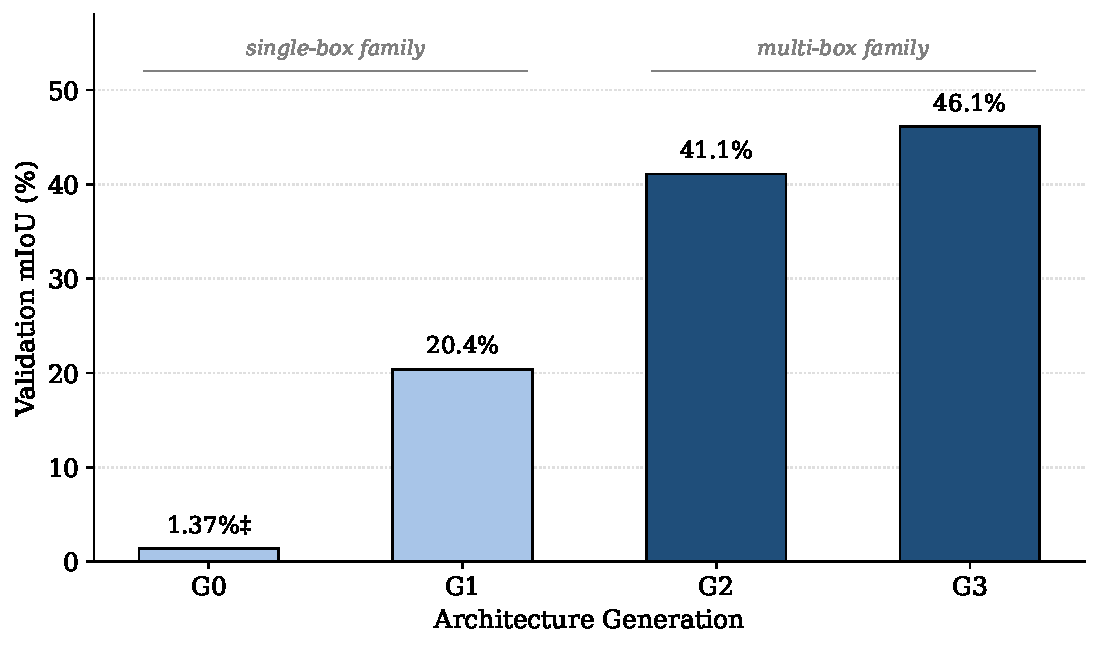
\includegraphics[width=0.7\textwidth]{chapter_4R/figures/arch_progression_chart.pdf}
    \caption[Validation mIoU progression across architecture generations.]{
        Validation \gls{miou} trajectory across the four design generations of \texttt{DetectorNX}. 
        The single-box-to-multi-box transition (G1 $\rightarrow$ G2) delivered the largest gain of $+20.7$~pp, while the high-resolution-backbone iteration (G2 $\rightarrow$ G3) resulted in a further $+5.0$~pp gain, leading to the final $46.1\%$ score.
        G0 is shown for completeness; its measurement strategy differs as documented in Table~\ref{tab:arch_progression_results}.
    }
    \label{fig:arch_progression_chart}
\end{figure}

The progression confirms that each architectural transition delivered a measurable improvement over its predecessor, with no plateau or regression at any step.
The largest single-step improvement ($+20.7$~pp, G1~$\rightarrow$~G2) comes from the introduction of the multi-box regression head, and the final gain ($+5.0$~pp, G2~$\rightarrow$~G3) reflects breaking the geometric-precision ceiling identified at the end of G2.

Validation \gls{miou} serves as the primary cross-generation metric, since it is the only quantitative measure collected across all four generations.
Additional generation-specific metrics corroborate the progression at finer granularity: the mean firing rate across all layers (G2: $<1.5\%$, G3: $\sim7.9\%$ mean post-\gls{frr}), and the documented failure modes (Constant Target Bias in G0; Super-Box artefact in G1) are presented in Section~\ref{sec:architectural_evolution}.

These results justify the selection of G3 as the canonical \texttt{DetectorNX-G3-SNN} architecture used for all subsequent baseline comparisons, energy benchmarking, and confidence-calibration analyses presented in the remainder of this chapter.